% !TeX root=../main.tex

\chapter{مقدمه}
% دستور زیر باعث عدم‌نمایش شماره صفحه در اولین صفحه‌ی این فصل می‌شود.
%\thispagestyle{empty}
\section{آشنایی با این راهنما}
حروف‌چینی پروژه کارشناسی، پایان‌نامه یا رساله یکی از موارد پرکاربرد استفاده از
\lr{\LaTeX}
و زی‌پرشین
\cite{Khalighi87xepersian}
است. یک پروژه، پایان‌نامه یا رساله، احتیاج به تنظیمات زیادی از نظر صفحه‌آرایی دارد که وقت زیادی از دانشجو می‌گیرد. به دلیل قابلیت‌های بسیار لاتک در حروف‌چینی، کلاسی با نام 
\lr{tehran-thesis}
برای حروف‌چینی پروژه‌ها، پایان‌نامه‌ها و رساله‌های دانشگاه تهران، بر مبنای کلاس مشابه
\lr{IUST-Thesis}
تهیه شده است. این کلاس و فایل‌های همراه آن به گونه‌ای طراحی شده است که مطابق با دستورالعمل نگارش و تدوین پایان‌نامه کارشناسی ارشد و دکتری پردیس دانشکده‌های فنی دانشگاه تهران
\cite{UTThesisGuide}
باشد.

دستورالعمل نگارش و تدوین پایان‌نامه دانشگاه تهران به دو مقوله می‌پردازد، اول قالب و چگونگی صفحه‌آرایی پایان‌نامه، مانند اندازه و نوع قلم بخشهای مختلف، چینش فصلها، قالب مراجع و مواردی از این قبیل و دوم محتوای هر فصل پایان‌نامه. 
درصورت استفاده از این کلاس، نیازی نیست که دانشجو نگران مقوله اول باشد و پس از تایپ مطالب خود می‌تواند آنها را با لاتک و ابزار آن اجرا کند تا پایان‌نامه خود را با قالب دانشگاه داشته باشد. همچنین با خواندن این راهنما از ملزومات محتوایی هر فصل پایان‌نامه نیز مطلع خواهد شد.

در ادامهٔ  مقدمهٔ این راهنما، ابتدا چگونگی استفاده از کلاس پایان‌نامه و فایل‌های همراه آن را به صورت فنی شرح می‌دهیم و سپس مطالبی را در مورد ویژگی‌های محتوایی فصل ۱ پایان‌نامه (یعنی مقدمه) خواهیم آورد.
بقیهٔ فصل‌های این راهنما، تنها خصوصیات محتوایی فصول مختلف پایان‌نامه را شرح خواهند داد. نهایتاً جهت یادآوری، در پیوست‌ها مطالبی دربارهٔ آشنایی با دستورات لاتک، مدیریت مراجع در لاتک و چگونگی رسم جداول، نمودارها و الگوریتم‌ها آورده خواهند شد.

\section{چگونگی استفاده از کلاس پایان‌نامه}
کلیه فایل‌های لازم برای حروف‌چینی با کلاس فوق، داخل پوشه‌ای به نام
\lr{tehran-thesis}
قرار داده شده است. توجه داشته باشید که برای استفاده از این کلاس باید فونت‌های
\lr{IRLotusICEE}
و
\lr{IRTitr}
را داشته باشید (که همراه با این کلاس هست و نیاز به نصب نیست).
قلم‌های
\lr{IRLotusICEE}
مستخرج از قلم‌های استاندارد
\lr{IRLotus}
شورای عالی اطلاع‌رسانی%
\footnote{
قلم‌های استاندارد
\lr{IRFonts}
از شورای عالی اطلاع‌رسانی، منطبق بر آخرین نسخه استاندارد یونیکد، استاندارد ملی ۶۲۱۹ و استاندارد
\lr{Adobe Glyph Naming}
هستند.
}
هستند که توسط دکتر بابایی‌زاده اصلاحاتی روی آنها صورت پذیرفته است: تبدیل صفر توپر به صفر توخالی (جهت تمایز بیشتر با نقطه) و اضافه شدن
\textit{\textbf{حالت توپر و ایرانیک توأم}}،
که این موارد در قلم‌های شورای عالی اطلاع‌رسانی وجود ندارد.

\subsection{این همه فایل؟!}
\label{muchFiles}
از آنجایی که یک پایان‌نامه یا رساله، یک نوشته بلند محسوب می‌شود، لذا اگر همه تنظیمات و مطالب پایان‌نامه را داخل یک فایل قرار بدهیم، باعث شلوغی و سردرگمی می‌شود. به همین خاطر، قسمت‌های مختلف پایان‌نامه یا رساله  داخل فایل‌های جداگانه قرار گرفته است. مثلاً تنظیمات پایه‌ای کلاس داخل فایل
\lr{tehran-thesis.cls}، 
قسمت مشخصات فارسی پایان‌نامه داخل 
\lr{faTitle.tex}،
مطالب فصل اول داخل 
\lr{chapter1.tex}
و تنظیمات قابل تغییر توسط کاربر داخل 
\lr{commands.tex}،
قرار داده شده است.
\textbf{
	فایل اصلی این مجموعه، فایل
	\lr{main.tex}
	می‌باشد.
}
% یعنی بعد از تغییر فایل‌های دیگر، برای دیدن نتیجه تغییرات، باید این فایل را اجرا کرد. بقیه فایل‌ها به این فایل، کمک می‌کنند تا بتوانیم خروجی کار را ببینیم.
اگر به فایل 
\lr{main.tex}
دقت کنید، متوجه می‌شوید که قسمت‌های مختلف پایان‌نامه، توسط دستورهایی مانند 
\lr{input}
و
\lr{include}
به فایل اصلی، یعنی 
\lr{main.tex}
معرفی شده‌اند.
با توجه به ساختار محتوایی دستورالعمل، در فایل
\lr{main.tex}
فرض شده که پایان‌نامه یا رساله شما، از ۵ فصل و تعدادی پیوست تشکیل شده است. با اینحال، شما می‌توانید به راحتی فصل‌ها و پیوست‌ها را با صلاحدید اساتید راهنما، کم و زیاد کنید. این کار، بسیار ساده است. فرض کنید بخواهید یک فصل دیگر هم به پایان‌نامه اضافه کنید. برای این کار، کافی است یک فایل با نام دلخواه مثلاً 
\lr{chapter6}
و با پسوند 
\lr{.tex}
بسازید و آن را داخل پوشه 
\lr{tehran-thesis}
قرار دهید و سپس این فایل را با دستور 
\verb!\include{chapter6}!
داخل فایل
\lr{main.tex}
 فراخوانی کنید.

\subsection{از کجا شروع کنم؟}
قبل از هر چیز، باید یک توزیع تِک مناسب مانند تک‌لایو
\lr{(TeXLive)}
را روی سیستم خود نصب کنید. تک‌لایو  را می‌توانید از 
 \href{http://www.tug.org/texlive}{سایت رسمی آن}%
\LTRfootnote{\lr{\url{http://www.tug.org/texlive}}}
 دانلود کنید یا مستقیماً از مخازن توزیع لینوکس خود بگیرید (مثلاً در اوبونتو با دستور
\LRE{\verb!sudo apt install texlive-full!}).
برای نصب تک‌لایو و اجرای اسناد زی‌پرشین می‌توانید از
\href{http://parsilatex.com/site/shop/}{دی‌وی‌دی مجموعه پارسی‌لاتک}%
\LTRfootnote{\lr{\url{http://parsilatex.com/site/shop/}}}
و فایل راهنمای موجود در آن هم کمک بگیرید.

برای تایپ و پردازش اسناد لاتک باید از یک ویرایشگر مناسب استفاده کنید. ویرایشگرهای
\lr{TeXWroks},
\lr{TeXstudio},
\lr{Texmaker}
و
\lr{BiDiTeXmaker}
بدین منظور تولید شده‌اند. می‌توان ویرایش‌گر 
 \href{https://bitbucket.org/srazi/biditexmaker3}{\lr{BiDiTeXmaker}}%
 \LTRfootnote{\lr{\url{https://bitbucket.org/srazi/biditexmaker3}}}
را که بویژه برای کار با زی‌پرشین و مطالب دوجهته بهبود یافته است، بهینه‌ترین ویرایشگر لاتک برای کار با اسناد فارسی عنوان کرد.
 
حال اگر نوشتن \پ اولین تجربه شما از کار با لاتک است، توصیه می‌شود که یک‌بار به صورت اجمالی، کتاب «%
\href{http://www.tug.ctan.org/tex-archive/info/lshort/persian/lshort.pdf}{مقدمه‌ای نه چندان کوتاه بر
\lr{\LaTeXe}}%
\LTRfootnote{\lr{\url{http://www.tug.ctan.org/tex-archive/info/lshort/persian/lshort.pdf}\hfill}}»
ترجمه دکتر مهدی امیدعلی را مطالعه کنید. این کتاب، کتاب بسیار کاملی است که خیلی از نیازهای شما در ارتباط با حروف‌چینی را برطرف می‌کند.
اگر تک لایو کامل را داشته باشید، این کتاب را هم دارید. کافیست در خط فرمان دستور زیر را بزنید:
\begin{latin}
	\texttt{texdoc lshort-persian}
\end{latin}
اگر عجله دارید، برخی دستورات پایه‌ای مورد نیاز در پیوست \ref{app:latexIntro} بیان شده‌اند.
 
بعد از موارد گفته شده، فایل 
\lr{main.tex}
و
\lr{faTitle.tex}
را باز کنید و مشخصات پایان‌نامه خود مثل نام، نام خانوادگی، عنوان پایان‌نامه و ... را جایگزین مشخصات موجود در فایل
\lr{faTitle.tex}
 کنید. نیازی نیست نگران چینش این مشخصات در فایل پی‌دی‌اف خروجی باشید، زیرا کلاس 
\lr{tehran-thesis}
همه این کارها را بطور خودکار برای شما انجام می‌دهد. در ضمن، موقع تغییر دادن دستورهای داخل فایل
\lr{faTitle.tex}
 کاملاً دقت کنید؛ این دستورها، خیلی حساس هستند و ممکن است با یک تغییر کوچک، موقع اجرا، خطا بگیرید. برای دیدن خروجی کار، فایل 
\lr{faTitle.tex}
 را 
\lr{Save}
(نه 
\lr{Save As})
کنید و بعد به فایل 
\lr{main.tex}
برگشته و آن را اجرا کنید%
\footnote{
	البته فایلهای این مجموعه به گونه‌ای هستند که در
	\lr{TeXWorks} یا
	\lr{TeXstudio}
	بدون بازگشت به فایل اصلی، می‌توانید سند خود را اجرا کنید.
}.
 حال اگر می‌خواهید مشخصات انگلیسی \پ را هم عوض کنید، فایل 
\lr{enTitle.tex}
را باز کنید و مشخصات داخلش را تغییر دهید.
%\RTLfootnote{
%برای نوشتن پروژه کارشناسی، نیازی به وارد کردن مشخصات انگلیسی پروژه نیست. بنابراین، این مشخصات بطور خودکار، نادیده گرفته می‌شود.
%}
در اینجا هم برای دیدن خروجی باید این فایل را ذخیره کرده، بعد به فایل 
\lr{main.tex}
برگشته و آن را اجرا کرد.

برای راحتی بیشتر، کلاس 
\lr{tehran-thesis.cls}
طوری طراحی شده است که کافی است فقط  یک‌بار مشخصات \پ را (در فایل‌های
\lr{faTitle.tex}
و
\lr{enTitle.tex})
وارد کنید و هر جای دیگر که این مشخصات لازم باشند، به طور خودکار درج می‌شوند. با این حال، اگر مایل بودید، می‌توانید تنظیمات موجود را تغییر دهید؛ گرچه، در صورتیکه کاربر مبتدی هستید و یا با ساختار فایل‌های  
\lr{cls}
 آشنایی ندارید، بهتر است به فایل 
\lr{tehran-thesis.cls}
دست نزنید.

نکته دیگری که باید به آن توجه کنید این است که در قالب آماده شده، سه گزینه به نام‌های
\lr{bsc}،
\lr{msc}
و
\lr{phd}
برای نوشتن پروژه، پایان‌نامه و رساله، در نظر گرفته شده است. بنابراین اگر قصد تایپ پروژهٔ کارشناسی، پایان‌نامهٔ کارشناسی ارشد یا رسالهٔ دکتری را دارید، به ترتیب باید از گزینه‌های
\lr{bsc}،
\lr{msc}
و
\lr{phd}
در فایل 
\lr{main.tex}
استفاده کنید. با انتخاب هر کدام از این گزینه‌ها، تنظیمات مربوط به آنها به طور خودکار، اعمال می‌شود.


\subsection[مطالب پایان‌نامه را چطور بنویسم؟]
{مطالب \پ را چطور بنویسم؟}
\subsubsection{نوشتن فصل‌ها}
همان‌طور که در بخش \ref{muchFiles} گفته شد برای جلوگیری از شلوغی، قسمت‌های مختلف \پ از جمله فصل‌ها، در فایل‌های جداگانه‌ای قرار داده شده‌اند. 
مثلاً اگر می‌خواهید مطالب فصل ۱ را تایپ کنید، باید فایل‌های 
\lr{main.tex}
و
\lr{chapter1.tex}
را باز کرده و مطالب خود را جایگزین محتویات داخل 
\lr{chapter1.tex}
نمایید. دقت شود که در ابتدای برخی فایلها دستوراتی نوشته شده است و از شما خواسته شده که آن دستورات را حذف نکنید.

%توجه کنید که همان‌طور که قبلاً هم گفته شد، تنها فایل قابل اجرا، 
%\lr{main.tex}
%است. لذا برای دیدن حاصل (خروجی) فایل خود، باید  
%\lr{chapter1.tex}
%را ذخیره کرده و سپس فایل 
%\lr{main.tex}
%را اجرا کنید.

نکته بسیار مهمی که در اینجا باید گفته شود این است که سیستم \lr{\TeX}، محتویات یک فایل تِک را به ترتیب پردازش می‌کند.  بنابراین، اگر مثلاً  دو فصل اول خود را نوشته و خروجی آنها را دیده‌اید و مشغول تایپ مطالب فصل ۳ هستید، بهتر است
که دو دستور 
\verb!% !TeX root=../main.tex

\chapter{مقدمه و بیان مسئله}
% دستور زیر باعث عدم‌نمایش شماره صفحه در اولین صفحه‌ی این فصل می‌شود.
%%%%%%%%%%%%%%%%%%%%% INTRO %%%%%%%%%%%%%%%%%%%%%
%\thispagestyle{empty}
\section{مقدمه}
ذخیره‌ی ایمن و مطمئن اطلاعات همواره یکی از چالش‌های اساسی در حوزه سیستم‌های کامپیوتری بوده‌است. امروزه با افزایش روزافزون و چشم‌گیر استفاده از سیستم‌های کامپیوتری و همچنین ظهور و بروز مفاهیمی همچون کلان‌داده این نیاز بیشتر حس می‌شود. به عنوان اولین راهکار می‌توان از توزیع‌شدگی نام‌برد. استفاده از یک پایگاه‌داده ایمن و مطمئن به منظور ذخیره‌سازی اطلاعات می‌تواند یک راهکار مناسب برای پاسخگویی به این نیاز برشمرده شود.

\subsection{زنجیره‌ی بلوکی}
با وجود اینکه، استفاده از یک پایگاه‌داده توزیع‌شده مناسب به نظر می‌رسد، اما در صورت اختلال در کارکرد هرکدام از گره‌های ذخیره‌سازی، روند دسترسی به داده‌ها با مشکل روبرو خواهدشد. در این میان برای حل این مشکل از افزونگی و تکنیک‌های موجود در ذخیره‌سازی استفاده می‌کنند. بدیهی‌است در این میان هرچه میزان افزونگی بیشتر شود، امکان بازیابی موثر اطلاعات افزایش یافته ولی سربار سیستم افزایش خواهد یافت. استفاده از یک شبکه همتا‌به‌همتا که در آن تمامی گره‌های عضو شبکه امکان اشتراک‌گذاری و استفاده از منابع یکدیگر را داشته باشند، می‌تواند به عنوان راهکار برای این چالش در نظر گرفته‌شود.


با استفاده از تمامی مفاهیم فوق در سال ۲۰۰۹ برای نخستین بار از یک مفهوم به نام زنجیره‌ی بلوکی رونمایی شد، که در آن داده‌ها در یک شبکه‌ی همتا‌به‌همتا ذخیره‌ می‌شدند. به منظور تامین امنیت ذخیره‌سازی داده‌ها، از فرآیند‌های مرتبط با رمزنگاری استفاده شده‌است. به عنوان برنامه‌ی کاربردی مرتبط با این پایگاه‌داده، از یک رمزارز استفاده‌شد. زنجیره‌ی بلوکی این قابلیت را در اختیار کاربران قرار داد تا با استفاده از آن بسترهای متعددی از قبیل رمزارز و قراردادهای هوشمند نیز ظهور و توسعه پیدا‌کنند.
\subsection{چالش‌های زنجیره‌ی بلوکی}
بدیهی است هر کدام از تکنولوژی‌های نوظهور با چالش‌هایی روبرو خواهندبود. زنجیره‌ی بلوکی نیز با چالش‌های جدی و اساسی‌ای روبرو است. چالش‌هایی از قبیل مقیاس‌پذیری، نشت اطلاعات و هزینه بالای سرویس به عنوان چالش‌های اساسی در این حوزه مطرح می‌شوند. برای هرکدام از چالش‌های نام‌برده شده راه‌حل‌های زیادی نام‌برده شده‌است. هریک از این راهکارها منتج به ایجاد شاخه‌های دیگری از زنجیره‌های بلوکی شده‌است.


در زنجیره‌بلوکی تمامی اطلاعات و داده‌ها باید در این بستر ذخیره شوند. با فراگیر شدن این پدیده نوظهور و اعمال آن برروی کاربردهایی از قبیل رمزارز و قراردادهای هوشمند، تمایل استفاده از این فناوری نوظهور به شدت افزایش یافته‌است. افزایش تعداد تراکنش‌ها در این بستر و همچنین افزایش روزافزون حجم معاملات در این بستر سبب شده تا این فناوری با چالش مقیاس‌پذیری بیشتر از سایر چالش‌ها روبرو باشد. در این پایان‌نامه سعی شده‌است تا چالش مقیاس‌پذیری با رویکرد بهبود روند ذخیره‌سازی بر روی ذخیره‌بلوکی اتریوم بهبود یابد.

%%%%%%%%%%%%%%%%%%%%% BACKGROUND %%%%%%%%%%%%%%%%%%%%%
\section{تاریخچه‌ای از موضوع تحقیق}
همان‌‌طور که اشاره شد، تمامی تراکنش‌های بر بستر زنجیره‌ی بلوکی می‌بایست در این زنجیره ذخیره شوند. با توجه به افزایش روزافزون تراکنش‌ها و معاملات صورت‌گرفته، حجم اطلاعات موردنیاز برای ذخیره‌سازی بر این بستر افزایش چشم‌گیری داشته است. این افزایش موجب به‌وجود‌آمدن چالش‌هایی از قبیل مقیاس‌پذیری، نشت اطلاعات و \dots شده‌است. در \cite{Lin2017}
تمامی چالش‌های موجود در این زمینه نام برده شده و در میان آن‌ها مقیاس‌پذیری به عنوان بزرگ‌ترین چالش پیش‌ روی زنجیر‌ه‌ی بلوکی شناخته شده‌است. 

در حال حاضر بسیاری از زنجیره‌های بلوکی مطرح، حجمی بالای ۱۰۰ گیگابایت را شامل می‌شوند. هنگامی که یک گره کاونده به شبکه زنجیره‌ی بلوکی اضافه می‌شود، ابتدا تمامی زنجیره‌ی قبلی را باربرداری و سپس شروع به حل فرآیند پیچیده‌ی محاسباتی می‌کند. این حجم بسیار بالا که به طور روزمره نیز مقدار آن افزوده می‌شود، یک چالش اساسی هنگام استفاده از زنجیره‌ی بلوکی است. \cite{Wang2018}
به منظور حل مشکل مقیاس‌پذیری موجود در زنجیره‌ی بلوکی، راهکارهای بسیاری از قبیل بهبود و بهینه‌سازی روند ذخیره‌سازی مطرح شده‌است.
در \cite{Kim2018} تمامی راهکارهای مطرح‌شده در حوزه‌ی مقیاس‌پذیری به پنج دسته‌ی کلی طبقه‌بندی شده‌اند؛ راهکارهایی که به اعمال تغییر بر روی عناصر زنجیره‌ی اصلی می‌پردازند، راهکارهایی با پردازش تراکنش‌ها در خارج از زنجیره‌ی اصلی، راهکارهایی با کمک‌گرفتن از زنجیره‌ی جانبی، راهکارهایی با ایجاد ساختار والد-مولد و راهکارهایی با فراهم کردن امکان ارتباط بین زنجیره‌های متعدد.
در ادامه به بررسی تعدادی از راهکارهای متداول استفاده‌شده در این حوزه می‌پردازیم.

\subsection{راهکارهای مبتنی بر بازطراحی زنجیره‌ی بلوکی}
هدف اصلی در این دسته از راهکارها تغییر ساختار زنجیره‌ی بلوکی و گره‌های آن به نحوی‌ست که نگه‌داری اطلاعات بهینه شود. بهینه‌سازی اطلاعات به منظور کاهش حجم موردنیاز برای ذخیره‌سازی هر کدام از داده‌ها معنا می‌شود. مهم‌ترین راهکار ارائه‌شده در این دسته، \cite{Eyal2015} است. در این روش، بلوک‌های سنتی به دو دسته‌ی بلوک‌های کلیدی برای انتخاب رهبر و ریزبلوک‌ها برای ذخیره‌سازی تراکنش‌ها تقسیم می‌شوند. در این طرحواره، عناصر کاونده سعی در کسب رهبری دارند. بلوک رهبر وظیفه‌ی تولید ریزبلاک‌ها را تا زمان انتخاب رهبر جدید بر عهده دارد. به این ترتیب زنجیره‌ی بلوکی بازطراحی شده و حجم ذخیره‌سازی در دست برای هر بلاک افزایش می‌یابد. 

\subsection{راهکارهای مبتنی بر اصلاح معیارهای ذخیره‌سازی}
این دسته از راهکارها، مشتمل بر روش‌هایی هستند که با بازتعریف‌کردن معیارهایی برای عناصر زنجیره‌‌ی بلوکی لزوم نگهداری هر بلوک برای گره‌های مختلف زنجیره را تعیین می‌نمایند. در راهکار ارائه‌شده در \cite{Bruce2017} تراکنش‌های قدیمی حذف شده و اعتبار آدرس‌ها در درخت حساب‌ها نگهداری می‌شود. به این ترتیب گره‌های شبکه لازم نیست برای بررسی درستی بلوک‌ها تمامی بلوک‌های زنجیره را نگهداری کنند. این روش به کاهش چشم‌گیر حجم اطلاعات دریافتی توسط گره‌های شبکه می‌انجامد. 

در راهکار دیگری که ذیل همین گروه بیان شده‌است، ‌می‌توان به \cite{VanDenHooff2014} اشاره کرد. این روش نیز بر ایجاد گره‌های سبک در شبکه تأکید دارد. ایده‌ی کلی این روش بر پایه‌ی برون‌سپاری محاسبات از طرف گره‌های سبک است. به منظور اطمینان از صحت نتایج محاسبات انجام‌شده، نتایج به‌دست‌آمده از کارگزارهای متفاوت با هم مقایسه می‌شوند.

\subsection{راهکارهای مبتنی بر بهبود ذخیره‌سازی}
راهکارهای ارائه‌شده در این دسته به طور مستقیم بر نحوه‌ی ذخیره‌سازی اطلاعات زنجیره‌ی بلوکی تمرکز دارند. در \cite{Pontiveros2018} یک روش فشرده‌سازی قراردادهای هوشمند بر بستر اتریوم پیشنهاد شده‌است. روش استفاده‌شده از تشابه کد اجرایی استفاده‌شده توسط قراردادهای هوشمند نگه‌داری‌شده در زنجیره بهره می‌گیرد. به این ترتیب با فشرده‌سازی اطلاعات، از حجم آن‌ها کاسته شده و در فضای ذخیره‌سازی صرفه‌جویی می‌شود.

%%%%%%%%%%%%%%%%%%%%% EXPLANATION %%%%%%%%%%%%%%%%%%%%%
\section{شرح مسئله تحقیق}
تحقیقات گسترده‌ای در حوزه حل چالش مقیاس‌پذیری در زنجیره‌ی بلوکی انجام شده‌است. در این پایان‌نامه سعی در کاهش حجم مصرفی برای ذخیره‌سازی زنجیره‌ی بلوکی داریم. می‌دانیم در تمامی زنجیره‌های بلوکی تمامی داده و رکوردها باید از ابتدا ذخیره شوند، همین امر سبب می‌شود تا حجم لازم برای ذخیره‌سازی این قسم پایگاه‌داده‌ها به شدت افزایش یابد. همان‌گونه که در بخش قبل اشاره‌شد، راهکارهای زیادی در این زمینه ارائه شده‌است. راهکار پیشنهادی از آنجا که به طور مستقیم بر نحوه ذخیره‌سازی تمرکز دارد، در گروه راهکارهای مبتنی بر بهبود ذخیره‌سازی تقسیم‌یندی می‌شود. 

%%%%%%%%%%%%%%%%%%%%% DESCRIPTION %%%%%%%%%%%%%%%%%%%%%
\section{تعریف موضوع تحقیق}
همان‌طور که اشاره‌شد، روش‌های بسیاری در حوزه حل مشکل‌ مقیاس‌پذیری زنجیره‌ی بلوکی انجام شده‌اند. در این پایان‌نامه راهکار ارائه شده به طور مشخص در گروه راهکارهای مبتنی بر بهبود ذخیره‌سازی قرار می‌گیرد. در روش ارائه شده مشکل مقیاس‌پذیری با استفاده از بهینه‌ ساختن روش ذخیره‌سازی انجام می‌شود. در روش ارائه شده تمامی بلوک‌های موجود در زنجیره‌ی بلوکی به نحوی فشرده شده و بلوک‌های فشرده‌شده با بلوک‌های اصلی جایگزین می‌شوند. می‌توان روش ارائه شده را یک روش بهبود مقیاس‌پذیری مبتنی بر فشرده‌سازی نیز بیان کرد.


در روش ارئه شده تمامی محتویات ذخیره‌شده در زنجیره‌های بلوکی فشرده‌شده فلذا حجم مورد نیاز برای ذخیره‌سازی این زنجیره کاهش خواهد یافت. بدیهی‌است انجام فرآیند ذخیره‌سازی با سربارهای زمانی روبرو خواهد بود. همچنین فرآیند فشرده‌سازی نیازمند صرف توان مصرفی و  اعمال بار پردازشی بر سیستم‌ خواهد بود. ذخیره‌سازی باید به صورتی باشد که میزان فشرده‌سازی توجیه سرباز زمانی و پردازشی سیستم‌ را بکند.

%%%%%%%%%%%%%%%%%%%%% GOALS %%%%%%%%%%%%%%%%%%%%%
\section{اهداف و آرمان‌های کلی تحقیق}
در روش ارائه‌شده، مشکل مقیاس‌پذیری با استفاده از روش‌های فشرده‌سازی مرتفع خواهدگردید. از آنجاییکه روش مورد نظر به صورت کاملا دقیق و جزئی به روش‌های فشرده‌سازی وابسته‌ خواهد‌بود، پس یک کاوش در حوزه روش‌های فشرده‌سازی می‌بایست انجام شود. روش‌های فشرده‌سازی به طور کلی برمبنای احتمال وقوع هرکدام از سمبل‌ها، یک عبارت را در نظر می‌گیرند. عبارت مورد نظر به طوریست که هرجه احتمال وقوع یک سمبل بیشتر باشد، آنگاه طول عبارت اختصاص یافته کوتاه‌تر خواهد بود. 


اکنون با در نظر گرفتن کاوش‌های انجام شده و بدست آوردن روش مورد نظر برای ذخیره‌سازی، می‌بایست الگوریتم ذخیره‌سازی را بر زنجیره‌بلوکی اعمال کرد. همان‌طور که اشاره‌شد، زنجیره‌ی بلوکی ذاتا از یک شبکه توزیع‌شده‌ی همتا‌به‌همتا استفاده می‌کند، روش ذخیره‌سازی به هیچ عنوان نباید متناقض با ذات زنجیره‌ی بلوکی باشد. این بدین معناست که روش ذخیره‌سازی ارائه شده به هیچ عنوان نباید به نحوی‌ باشد که زنحیره را به سمت یک شبکه متمرکز سوق دهد.

%%%%%%%%%%%%%%%%%%%%% METHOD %%%%%%%%%%%%%%%%%%%%%
\section{روش انجام تحقیق}
زنجیره‌ی بلوکی را می‌توان به عنوان پایگاه‌داده برروی کاربردهای مختلفی بکار گرفت. یکی از مهمترین کاربردهای مورد استفاده از زنحیره‌ی بلوکی استفاده به عنوان پایگاه‌داده‌‌ای مطمئن برای حفظ و ذخیره‌سازی قراردا‌د‌های هوشمند است. در این پایان‌نامه به منظور ایجاد یک زنجیره‌ی بلوکی از زنجیره‌ی بلوکی مبتنی بر اتریوم استفاده ‌شده‌است.

فرآیند فشرده‌سازی همراه با سربار زمانی و صرف توان مصرفی خواهدبود. با در نظر گرفتن این امر می‌توان روش ارائه‌شده را از ابعاد مختلف مورد بررسی و واکاوی قرار داد. روش ارائه‌شده می‌تواند به صور مختلفی در نظر گرفته‌شود این بدین معناست که روش پیشنهادی می‌تواند با توجه به محدودیت‌های موجود و در نظر گرفته‌شده برای هر سیستم خود را تطبیق دهد.

ذیل برگزاری آزمایشات برای آزمودن روش پیشنهادی، پارامترهایی از قببل میزان فشرده‌سازی، سربار زمانی و همچنین توان مصرفی مورد آزمون قرار گرفته‌اند. روش پیشنهادی یک روش منعطف در برابر محدودیت‌ها است. با توجه به محدودیت‌های موجود در این بخش می‌تواند خود را تطبیق دهد.

%%%%%%%%%%%%%%%%%%%%% STRUCTURE %%%%%%%%%%%%%%%%%%%%%
\section{ساختار پایان‌نامه}
در فصل دوم مفاهیم و تعاریف اساسی مربوط به زنجیره‌ی بلوکی، قراردادهای هوشمند و به طور خاص اتریوم ارائه می‌شود. هم‌چنین به مفاهیم و اجزای اساسی پژوهش که چالش مقیاس‌پذیری و راه حل فشرده‌سازی هستند پرداخته خواهدشد.
فصل سوم دربرگیرنده‌ی توضیحات مربوط به راه حل پیشنهادی و ابزارهای مورداستفاده است. در این فصل معیارهای موردنظر برای ارزیابی راه‌حل عنوان خواهند شد.
در فصل چهارم نتایج و نمودارهای حاصل از بررسی انجام‌شده ارائه می‌شوند و نتایج به‌دست‌آمده تحلیل خواهندشد. در این فصل ویژگی‌های هریک از روش‌ها مورد بررسی بیان خواهد شد.
در نهایت، در فصل پنجم، نتیجه‌گیری‌های کلی حاصل‌شده در این پژوهش، نوآوری‌های انجام‌شده و محدودیت‌ها مورد بحث قرار می‌گیرد و پیشنهادهایی برای ادامه‌ی این پژوهش ارائه خواهد شد.!
و
\verb!% !TeX root=../main.tex
\chapter{مروری بر مطالعات انجام شده}
%\thispagestyle{empty} 
\section{مقدمه}
هدف از این فصل که با عنوان‌های  «مروری بر ادبیات موضوع%
\LTRfootnote{Literature Review}»،
«مروری بر منابع» و یا «مروری بر پیشینه تحقیق%
\LTRfootnote{Background Research}»
معرفی می‌شود، بررسی و طبقه‌بندی یافته‌های تحقیقات دیگر محققان در سطح دنیا و تعیین و شناسایی خلأهای تحقیقاتی است. آنچه را که تحقیق شما به دانش موجود اضافه می‌کند، مشخص کنید. طرح پیشینه تحقیق%
\LTRfootnote{Background Information}
یک مرور محققانه است و تا آنجا باید پیش برود که پیش‌زمینهٔ تاریخی مناسبی از تحقیق را بیان کند و جایگاه تحقیق فعلی را در میان آثار پیشین نشان دهد. برای این منظور منابع مرتبط با تحقیق را بررسی کنید، البته نه آنچنان گسترده که کل پیشینه تاریخی بحث را در برگیرد. برای نوشتن این بخش:
\begin{itemize}
	\item
	دانستنی‌های موجود و پیش‌زمینهٔ تاریخی و وضعیت کنونی موضوع را چنان بیان کنید که خواننده بدون مراجعه به منابع پیشین، نتایج حاصل از مطالعات قبلی را درک و ارزیابی کند.
	\item
	نشان دهید که بر موضوع احاطه دارید. پرسش تحقیق را همراه بحث و جدل‌ها و مسائل مطرح شده بیان کنید و مهم‌ترین تحقیق‌های انجام شده در این زمینه را معرفی نمائید.
	\item
	ابتدا مطالب عمومی‌تر و سپس پژوهش‌های مشابه با کار خود را معرفی کرده و نشان دهید که تحقیق شما از چه جنبه‌ای با کار دیگران تشابه یا تفاوت دارد.
	\item
	اگر کارهای قبلی را خلاصه کرده‌اید، از پرداختن به جزئیات غیرضروری بپرهیزید. در عوض، بر یافته‌ها و مسائل روش‌شناختی مرتبط و نتایج اصلی تأکید کنید و اگر بررسی‌ها و منابع مروری عمومی دربارهٔ موضوع موجود است، خواننده را به آنها ارجاع دهید.
\end{itemize}

\section{تعاریف، اصول و مبانی نظری}
این قسمت ارائهٔ خلاصه‌ای از دانش کلاسیک موضوع است. این بخش الزامی نیست و بستگی به نظر استاد راهنما دارد.

\section{مروری بر ادبیات موضوع}
در این قسمت باید به کارهای مشابه دیگران در گذشته اشاره کرد و وزن بیشتر این قسمت بهتر است به مقالات ژورنالی سال‌های اخیر (۲ تا ۳ سال) تخصیص داده شود. به نتایج کارهای دیگران با ذکر دقیق مراجع باید اشاره شده و جایگاه و تفاوت تحقیق شما نیز با کارهای دیگران مشخص شود. استفاده از مقالات ژورنال‌های معتبر در دو یا سه سال اخیر، می‌تواند به اعتبار کار شما بیافزاید.

\section{نتیجه‌گیری}
‌در نتیجه‌گیری آخر این فصل، با توجه به بررسی انجام شده بر روی مراجع تحقیق، بخش‌های قابل گسترش و تحقیق در آن حیطه و چشم‌اندازهای تحقیق مورد بررسی قرار می‌گیرند.	در برخی از تحقیقات، نتیجه نهایی فصل روش تحقیق، ارائهٔ یک چارچوب کار تحقیقی 
\lr{(research framework)}
است.!
را در فایل 
\lr{main.tex}،
غیرفعال%
\footnote{
برای غیرفعال کردن یک دستور، کافی است در ابتدای آن، علامت درصد انگلیسی (\%) بگذارید.
}
 کنید. در غیر این صورت، ابتدا مطالب دو فصل اول پردازش شده و سپس مطالب فصل ۳ پردازش می‌شود که این کار باعث طولانی شدن زمان پردازش می‌گردد. هر زمان که خروجی کل \پ را خواستید، تمام فصل‌ها را دوباره در
\lr{main.tex}
فعال نمائید.
بدیهتاً لازم نیست فصل‌های \پ را به ترتیب تایپ کنید. مثلاً می‌توانید ابتدا مطالب فصل ۳ را تایپ نموده و سپس مطالب فصل ۱ را تایپ کنید. 
\subsubsection{مراجع}
برای وارد کردن مراجع \پ کافی است فایل 
\lr{MyReferences.bib}
را باز کرده و مراجع خود را به شکل اقلام نمونهٔ داخل آن، وارد کنید.  سپس از \lr{bibtex} برای تولید مراجع با قالب مناسب استفاده نمائید. برای توضیحات بیشتر بخش \ref{Sec:Ref} از پیوست \ref{app:latexIntro} و نیز پیوست \ref{app:refMan} را ببینید.

\subsubsection{واژه‌نامه فارسی به انگلیسی و برعکس}
برای وارد کردن معادل فارسی اصطلاحات لاتین در متن و تهیه فهرست واژه‌نامه از آنها، از بستهٔ
\lr{glossaries}
و نرم‌افزار
\lr{xindy}
استفاده می‌شود. بدین منظور کافی است اصطلاحات لاتین و ترجمهٔ آنها را در فایل
\lr{words.tex}
وارد کرده و هر جای متن که خواستید با دستورات
\verb|gls{label}|
یا \verb|glspl{label}|
معادل فارسی مفرد یا جمع یک اصطلاح را بیاورید.

مثلا در اینجا، واژهٔ
«\gls{Action}»
برای بار اول و دوباره
«\gls{Action}»
برای بار دوم در متن ظاهر شده است.
جهت توضیحات بیشتر به پیوست
\ref{app:refMan}
مراجعه کنید.
\subsubsection{نمایه}
برای وارد کردن نمایه، باید از 
\lr{xindy}
استفاده کنید. 
%زیرا 
%\lr{MakeIndex}
%با حروف «گ»، «چ»، «پ»، «ژ» و «ک» مشکل دارد و ترتیب الفبایی این حروف را رعایت نمی‌کند. همچنین، فاصله بین هر گروه از کلمات در 
%\lr{MakeIndex}،
%به درستی رعایت نمی‌شود که باعث زشت شدن حروف‌چینی این قسمت می‌شود. 
راهنمای چگونگی کار با 
\lr{xindy} 
را می‌توانید در ویکی پارسی‌لاتک و یا مثالهای موجود در دی‌وی‌دی «مجموعه پارسی‌لاتک»، پیدا کنید.

\subsection{اگر سوالی داشتم، از کی بپرسم؟}
برای پرسیدن سوال‌های خود موقع حروف‌چینی با زی‌پرشین، می‌توانید به
\href{http://qa.parsilatex.com}{سایت پرسش و پاسخ پارسی‌لاتک}%
\LTRfootnote{http://qa.parsilatex.com}
یا
\href{http://forum.parsilatex.com}{بایگانی تالارگفتگوی قدیمی پارسی‌لاتک}%
\LTRfootnote{http://forum.parsilatex.com}
مراجعه کنید. شما هم می‌توانید روزی به سوال‌های دیگران در اینترنت جواب دهید.
بستهٔ زی‌پرشین و بسیاری از بسته‌های مرتبط با آن مانند
\lr{bidi} و
\lr{Persian-bib}،
مجموعه پارسی‌لاتک، مثالهای مختلف موجود در آن، قالب پایان‌نامه دانشگاههای مختلف و سایت پارسی‌لاتک همه به صورت داوطلبانه توسط افراد گروه پارسی‌لاتک و گروه
\lr{Persian TeX}
و بدون هیچ کمک مالی انجام شده‌اند. کار اصلی نوشتن و توسعه زی‌پرشین توسط آقای وفا خلیقی انجام شده است که این کار بزرگ را به انجام رساندند.
اگر مایل به کمک به گروه پارسی‌لاتک هستید به سایت این گروه مراجعه فرمایید:
\begin{center}
	\url{http://www.parsilatex.com}
\end{center}

\section{محتویات فصل اول یک پایان‌نامه}
فصل اول یک پایان‌نامه باید به مقدمه یا کلیات تحقیق بپردازد.
هدف از فصل مقدمه%
\LTRfootnote{Introduction}،
شرح مختصر مسأله تحقیق، اهمیت و انگیزه محقق از پرداختن به آن موضوع، بهمراه اشاره‌ای کوتاه به روش و مراحل تحقیق است. مقدمه، اولین فصل از ساختار اصلی \پ بوده و زمینه اطلاعاتی لازم را برای خواننده فراهم می‌آورد. در طول مقدمه باید سعی شود موضوع تحقیق با زبانی روشن، ساده و بطور عمیق و هدفمند به خواننده معرفی شود. این فصل باید خواننده را مجذوب و اهمیت موضوع تحقیق را آشکار سازد. در مقدمه باید با ارائهٔ سوابق، شواهد تحقیقی و اطلاعات موجود (با ذکر منبع) با روشی منظم، منطقی و هدف‌دار، خواننده را جهت داد و به سوی راه حل مورد نظر هدایت کرد. مقدمه مناسب‌ترین جا برای ارائهٔ اختصارات و بعضی توضیحات کلی است، توضیحاتی که شاید نتوان در مباحث دیگر آنها را شرح داد.

مقدمه، یکی از ارکان اساسی و اصلی پایان نامه است که مهمترین قسمت‌های آن عبارتند از: 

\subsection{عنوان تحقیق} 
باید شناختی دقیق و روشن از حوزهٔ موضوع تحقیق را عرضه دارد و خالی از هرگونه ابهام و پیچیدگی باشد.

\subsection{مسأله تحقیق}
وظیفه اصلی مقدمه بیان این مطلب به خواننده است که چرا انجام تحقیق را به عهده گرفته‌اید. اگر دلیل شما برای انجام این کار پاسخگویی به سؤال مورد علاقه‌تان است، با مشکل زیادی روبه‌رو نخواهید بود. یکی از بهترین روش‌ها برای نوشتن مقدمهٔ یک پایان‌نامه، طرح پرسش یا پرسش‌هایی مهم و اساسی است که کار تحقیقاتی شما از آغاز تا پایان قصد پاسخ دادن به آن را دارد. گاهی می‌توانید ابتدا اهمیت موضوع را بیان و سپس پرسش خود را در آن موضوع مطرح کنید.

\subsection{تاریخچه‌ای از موضوع تحقیق}
به طور کلی تشریح روندهای تحقیقاتی در محدودهٔ مورد مطالعه، مستلزم ارجاع به کارهای دیگران است. بعضی از نویسندگان برای کارهای دیگران هیچ اعتباری قائل نمی‌شوند و در مقابل، بعضی دیگر از نویسندگان در توصیف کارهای دیگران، بسیار زیاده‌روی می‌کنند. اکثر مواقع، ارجاع به مقالات دو سال قبل از کارتان، بهتر از نوشتن سطرهای مرجع است. در این قسمت باید به طور مختصر به نظرات و تحقیقات مربوط به موضوع و یا مسائل و مشکلات حل نشده در این حوزه و همچنین توجه و علاقه جامعه به این موضوع، اشاره شود.

\subsection{تعریف موضوع تحقیق}
در این قسمت محقق، موضوع مورد علاقه و یا نیاز احساس شدهٔ خود را در حوزه تحقیق بیان می‌دارد و عوامل موجود در موقعیت را تعریف و تعیین می‌کند.

\subsection{هدف یا هدف‌های کلی و آرمانی تحقیق}
این قسمت باید با جملات مثبت و کلی طرح شود و از طولانی شدن مطالب پرهیز شود.

\subsection{روش انجام تحقیق}
در این قسمت، پژوهشگر روش کاری خود را بیان می‌دارد و شیوه‌های گوناگونی را که در گردآوری مطالب خود بکار برده، ذکر می‌کند. همچنین اگر روش آماری خاصی را در تهیه و تدوین اطلاعات به کار برده است، آن شیوه را نیز اینجا بیان می‌کند.

\subsection{نوآوری، اهمیت و ارزش تحقیق}
در این قسمت، در مورد نوآوری علمی و عملی تحقیق که محقق به آن دست خواهد یافت، بحث می‌شود. ممکن است لازم باشد تا برخی نمودارهای خلاصه در این بخش استفاده شوند. به عنوان مثال، نموداری از مقاله
\cite{kim2016integrated}
در شکل
\ref{fig:sampleDiagram}
آمده است.
\begin{figure}[ht]
	\centerline{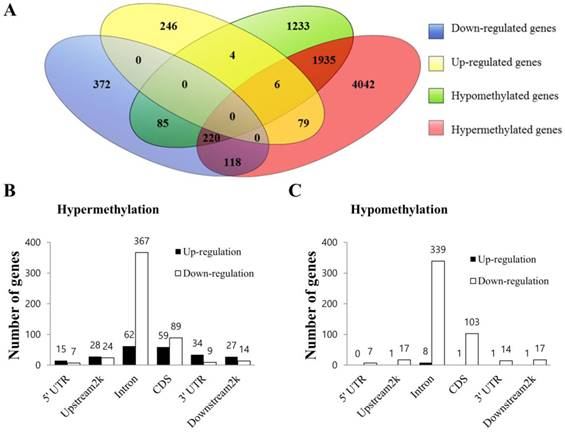
\includegraphics[width=0.8\textwidth]{journal-of-cancer_sample-result}}
	\caption{یک نمونه نمودار خلاصه برای نمایش نوآوری در نتایج
		%\cite{kim2016integrated}
	}
	\label{fig:sampleDiagram}
\end{figure}\\
طبیعتاً به صلاحدید نگارنده، شکل‌ها و نمودار‌ها می توانند در بخش های مختلف، خصوصا فصل
\ref{chap:results}
مورد استفاده قرار گیرند.

\subsection{تعریف واژه‌ها (اختیاری)}
در این قسمت محقق باید واژه‌هایی را که ممکن است برای خواننده آشنا نباشد، تعریف کند.

\subsection{خلاصه فصل‌ها}
در آخرین قسمتِ فصل اول پایان‌نامه، خلاصه‌ای اشاره‌وار از فصل‌های آتی آورده می‌شود تا خواننده بتواند تصویری واضح از دیگر قسمت‌های پایان‌نامه در ذهن خود ترسیم کند.

\section{جمع‌بندی}
در این فصل به دو مقولهٔ نحوه استفاده از قالب \پ دانشگاه تهران و نیز ویژگی‌هایی که محتویات فصل اول پایان‌نامه (یعنی مقدمه) باید داشته باشند، پرداخته شد. با توجه به اینکه این راهنما نحوه استفاده از قالب را شرح داده، ملزومات محتوایی هر فصل پایان‌نامه را توضیح می‌دهد و در پیوست‌ها نیز نحوهٔ کار با لاتک را یادآوری خواهد کرد، بنابراین مطالعهٔ کامل آن مقداری وقت شما را خواهد گرفت؛ اما مطمئن باشید از اتلاف وقت شما در ادامه کارتان تا حد زیادی جلوگیری خواهد کرد. در نوشتن متن حاضر سعی شده است علاوه بر ایجاد یک قالب لاتک برای پایان‌نامه‌های دانشگاه تهران، نکات محتوایی هر فصل نیز گوشزد گردد. طبیعتاً برای نگارش پایان‌نامهٔ خود می‌بایست مطالب تمام فصل‌ها را خودتان بازنویسی کنید.

در ادامهٔ این راهنما، تنها فصل‌هایی که یک پایان‌نامه باید داشته باشد و نیز خصوصیات یا ساختاری که محتویات هر فصل باید از آنها برخوردار باشد%
\footnote{از روی فایل «تمپلیت نگارش و تدوین پایان‌نامه \cite{UTThesisGuide}»}،
آورده می‌شوند. نهایتاً  در پیوست‌ها، مطالبی در باب یادآوری دستورات لاتک، نحوه نوشتن فرمول‌ها، تعاریف، قضایا، مثال‌ها، درج تصاویر، نمودارها، جداول و الگوریتم‌ها و نیز مدیریت مراجع، آمده است.

همچنین توصیه اکید دارم که رفع خطاهایی که احتمالاً با آنها مواجه می‌شوید را به آخر موکول نفرمایید و به محض برخورد با خطا، آن را اشکال‌زدایی و برطرف نمائید.